\subsection{Algoritmo Evolutivo para la Búsqueda de Caos}

Se propuso emplear un método heurístico para buscar parámetros del sistema implementado de tal forma que se maximice la caoticidad de su salida.
La idea es utilizar al MLE como la \textit{fitness function} de un algoritmo evolutivo, mediante el cual se busca maximizarla.
Este algoritmo tiene la ventaja que realiza una búsqueda inteligente mediante el empleo de un algoritmo genético, lo que minimiza el tiempo de cómputo.

Los algoritmos evolutivos son algoritmos de optimización metaheurísticos basados en poblaciones, que utilizan mecanismos inspirados en la biología tales como mutación, cruza, selección natural y supervivencia del más apto para refinar un conjunto de soluciones candidatas en forma iterativa\cite{Weise2009}.

Las entidades que representan posibles soluciones al problema son llamados \textit{cromosomas} y el grupo de cromosomas es llamados \textit{población inicial}.
Desde la población inicial, o los primeros padres, se genera un hijo mediante el cruce entre ellos.
Luego, ellos son mutados en forma aleatoria para crear la próxima generación.
Cada generación es comparada con la previa para descartar los ``peor adaptados'' y así los coeficientes (cromosomas) mutan hacia los ``mejor adaptados''.

Cuando se aplican estos algoritmos en funciones continuas, siempre convergen hacia el máximo local.
Sin embargo, si el espacio de coeficientes es fractal, existen áreas bien definidas en donde la función objetivo es positiva, negativa, cero o no existente.
Este es el caso cuando la función a maximizar es el MLE y el espacio de exploración es el de los parámetros de un sistema.

\subsubsection{Resultados}

Para evaluar la viabilidad del método, se generó el siguiente algoritmo y se probó sobre el mapa Logístico.

En la Figura \ref{fig:diagramaflujo1} podemos ver el diagrama de flujo principal.
El bloque \textit{Evolution} fue descompuesto en otro sub-diagrama para simplificar la descripción.
Este segundo diagrama puede verse en la Figura \ref{fig:diagramaflujo2}, esta subrutina maneja la evolución de los parámetros.
%
\begin{figure}
	\centering
	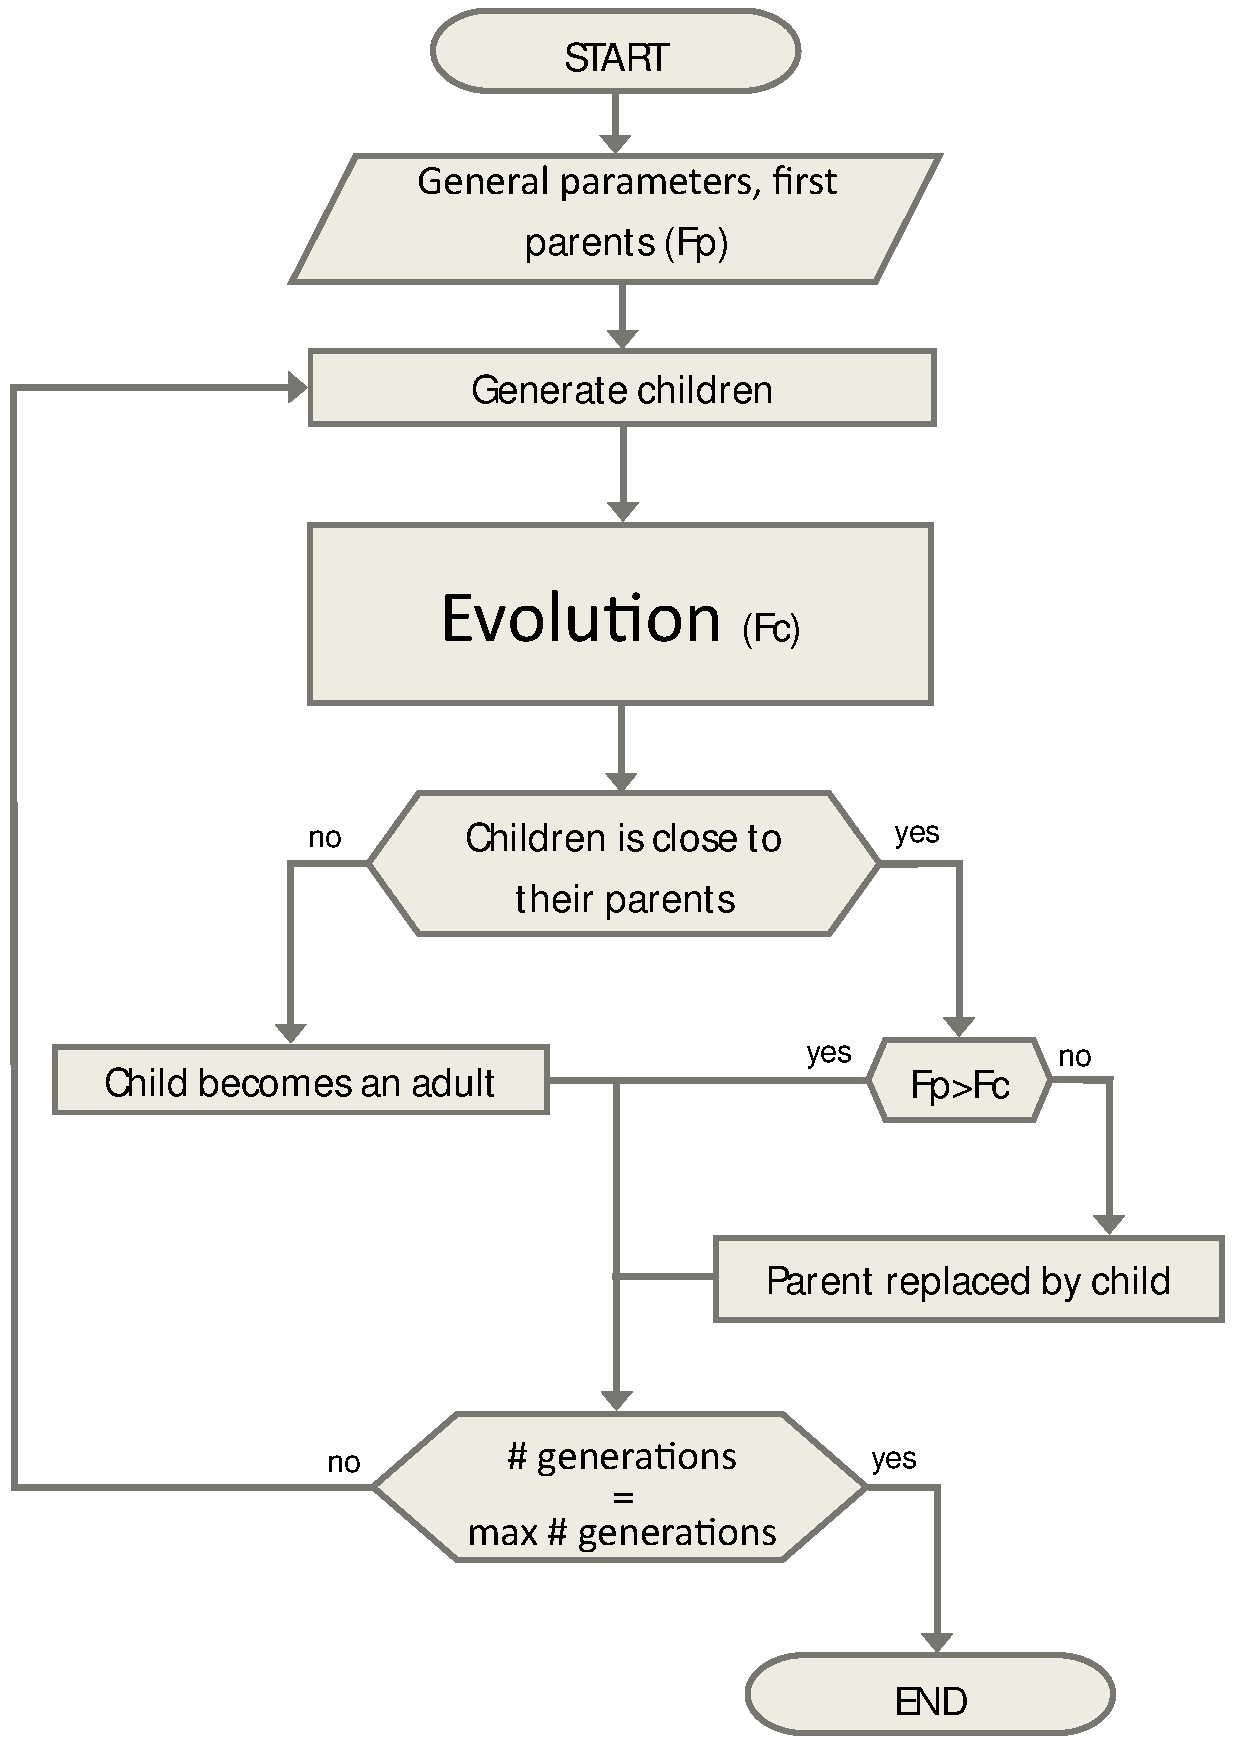
\includegraphics[width=0.9\columnwidth]{main_flowchart}\\
	\caption{Diagrama de flujo principal.}
	\label{fig:diagramaflujo1}
\end{figure}
%
\begin{figure}
	\centering
	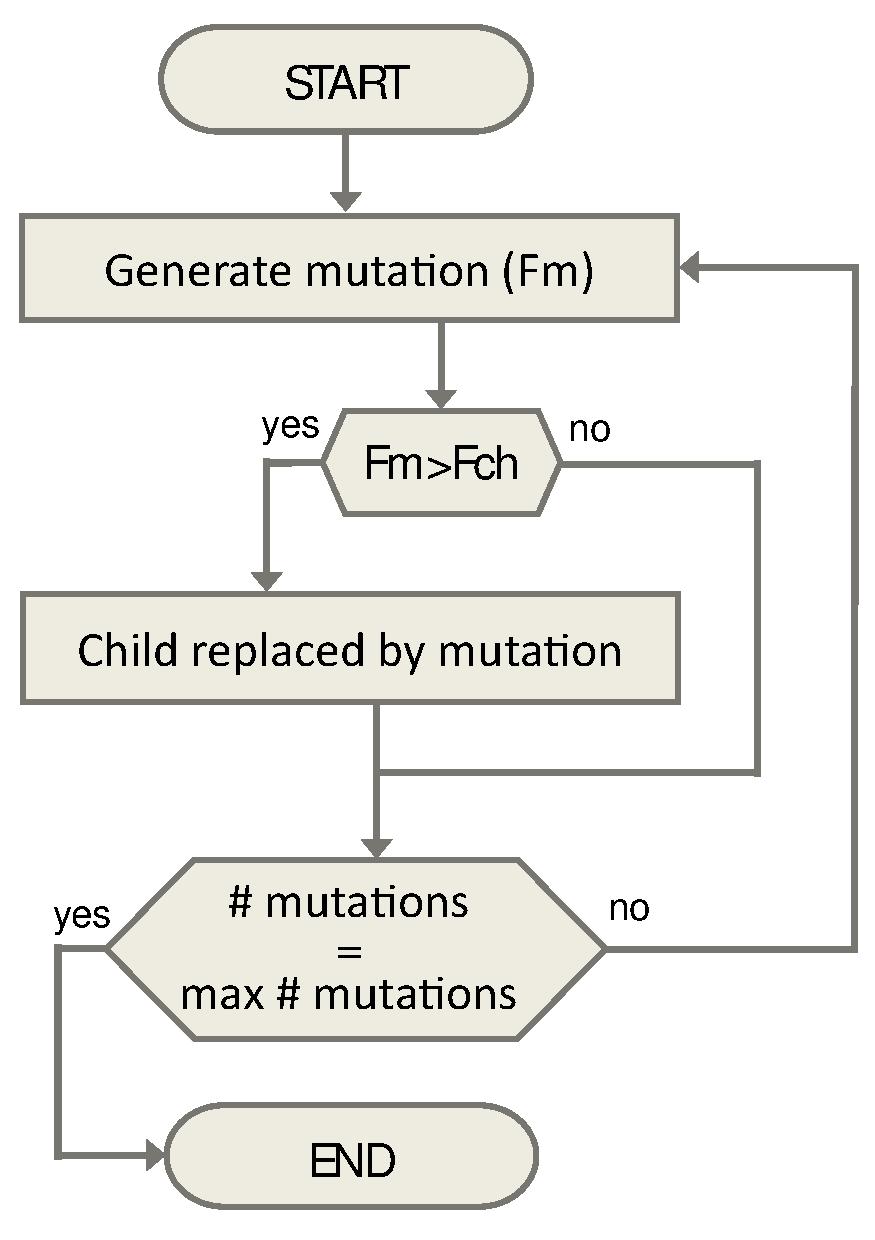
\includegraphics[width=0.56\columnwidth]{evolution_flowchart.pdf}\\
	\caption{Diagrama de flujo del bloque \textit{Evolution}.}\label{fig:diagramaflujo2}
\end{figure}

El algoritmo comienza con una inicialización general de parámetros como el número máximo de generaciones $max\_gen$, el número máximo de mutaciones $max\_mut$ y el número máximo de cambios en cada mutación $max\_stem$.
Luego se definen los primeros dos padres, ellos definirán los márgenes de búsqueda.
Además se calcula su \textit{fitness function} $F_p$.
A partir de este punto se itera la segunda generación, se elige en forma aleatoria un valor de parámetro $r$ con una distribución aleatoria entre los primeros dos padres, generando un nuevo hijo.
Luego este hijo entra en la subrutina \textit{Evolution} cuya salida es el valor de $r$ evolucionado y su correspondiente \textit{fitness function} $F_c$.

Luego se evalúa si este hijo evolucionó muy cerca de sus padres o no.
Si la distancia entre ellos es más grande que el parámetro $max\_hop$, entonces este hijo es considerado como adulto, en caso contrario debe competir con su padre más cercano sobreviviendo el más apto.

Este proceso se repite hasta que se llega al máximo número de  generaciones $max\_gen$.
El grupo final de adultos es la solución al problema de buscar los máximos MLE locales.

La subrutina \textit{Evolution} de la Figura \ref{fig:diagramaflujo2} es un algoritmo muy simple basado en mutaciones.
El primer paso es generar una mutación del hijo con una probabilidad uniformemente distribuida entre $\pm max\_step$, también se calcula su \textit{fitness function} $F_m$, que se compara con la del individuo original $Fc$.
Entonces sobrevive el mejor adaptado para dar lugar a la siguiente mutación.
Este procedimiento se repite hasta que se llega al máximo número de mutaciones $max\_mut$.

Como resultado podemos ver el $MLE$ del mapa Logístico en función de su único parámetro $r$ en la Figura \ref{fig:resultadoAlgorithm}.
La línea continua muestra el $MLE$ con un paso muy fino de $r$ ($\Delta r = 0.01$), mientras que los puntos destacados son el resultado del algoritmo propuesto.
%
\begin{figure}
	\centering
	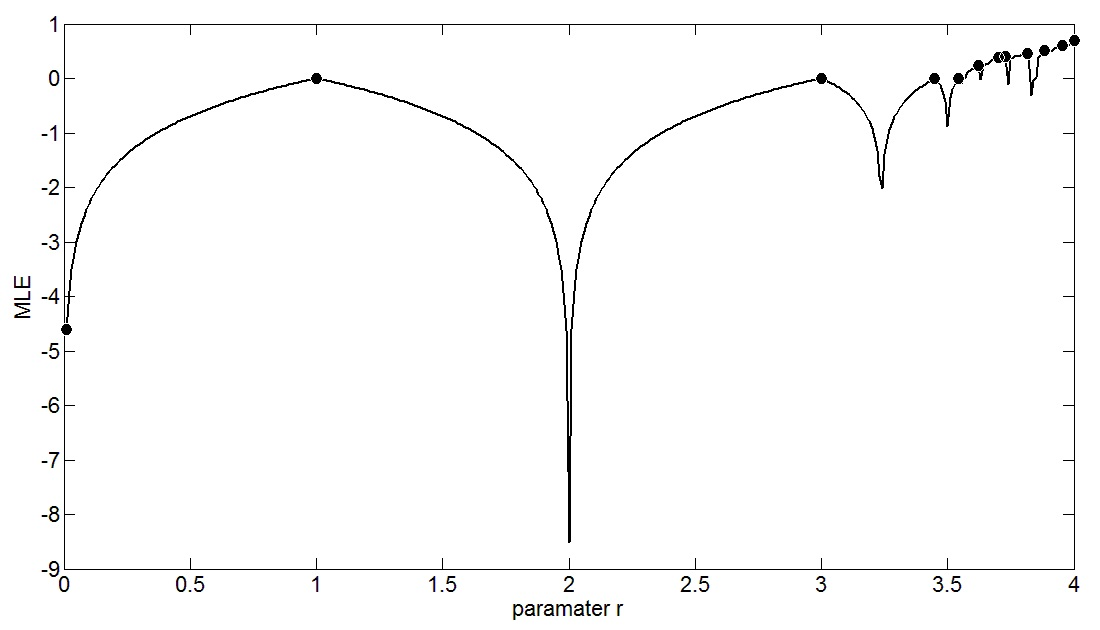
\includegraphics[width=1\columnwidth]{EvolutivoVSExaustivo.jpg}\\
	\caption{Resultados del algoritmo evolutivo para el mapa Logístico, los puntos son los resultados del algoritmo.}\label{fig:resultadoAlgorithm}
\end{figure}

El bloque que calcula el $MLE$ fue sintetizado y verificado experimentalmente en un Altera CYCLONE III FPGA y los resultados de la compilación se muestran en la Figura \ref{fig:compilacion}.
Los resultados del \textit{Timing Analysis} reportan que la máxima frecuencia es de $84.95MHz$.
El reporte de compilación muestra que la utilización de la lógica no excede el $20\%$, es decir un total de $20307$ de elementos lógicos, $54\%$ de los bits de memoria totales y $8\%$ de los multiplicadores embebidos.
%
\begin{figure}
	\centering
	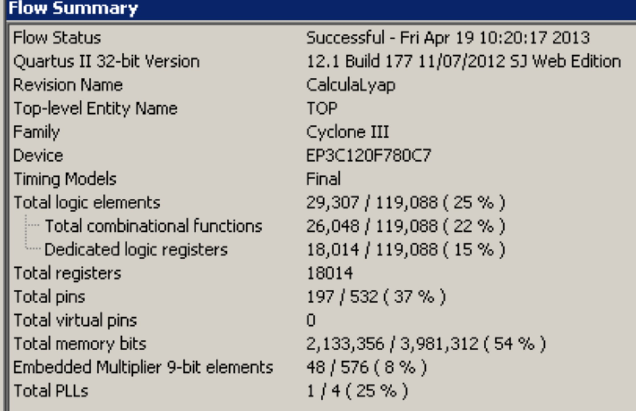
\includegraphics[width=.75\columnwidth]{compilacion.pdf}\\
	\caption{Reporte de compilación de la implementación del calculo del MLE.}\label{fig:compilacion}
\end{figure}

En la Figura \ref{fig:st} se muestra la salida del Signal Tap, esta herramienta permite tomar muestras directamente desde la placa en donde es implementado el algoritmo.
La señal \textit{salida} es la suma de los $MLE$ luego de cada iteración.
La segunda señal llamada \textit{cuenta\_sal} corresponde a la sumatoria actual.
Finalmente, cada flanco descendente de la señal \textit{listoD1} indica que la salida es un dato válido.
La salida fue procesada con Matlab para obtener la curva mostrada en la Figura\ref{fig:lyapu}.
El valor del MLE en la iteración $250~000$ es $0.1415$, lo que es consistente con el MLE obtenido con Matlab para el mapa Logístico.
%
\begin{figure*}
	\centering
	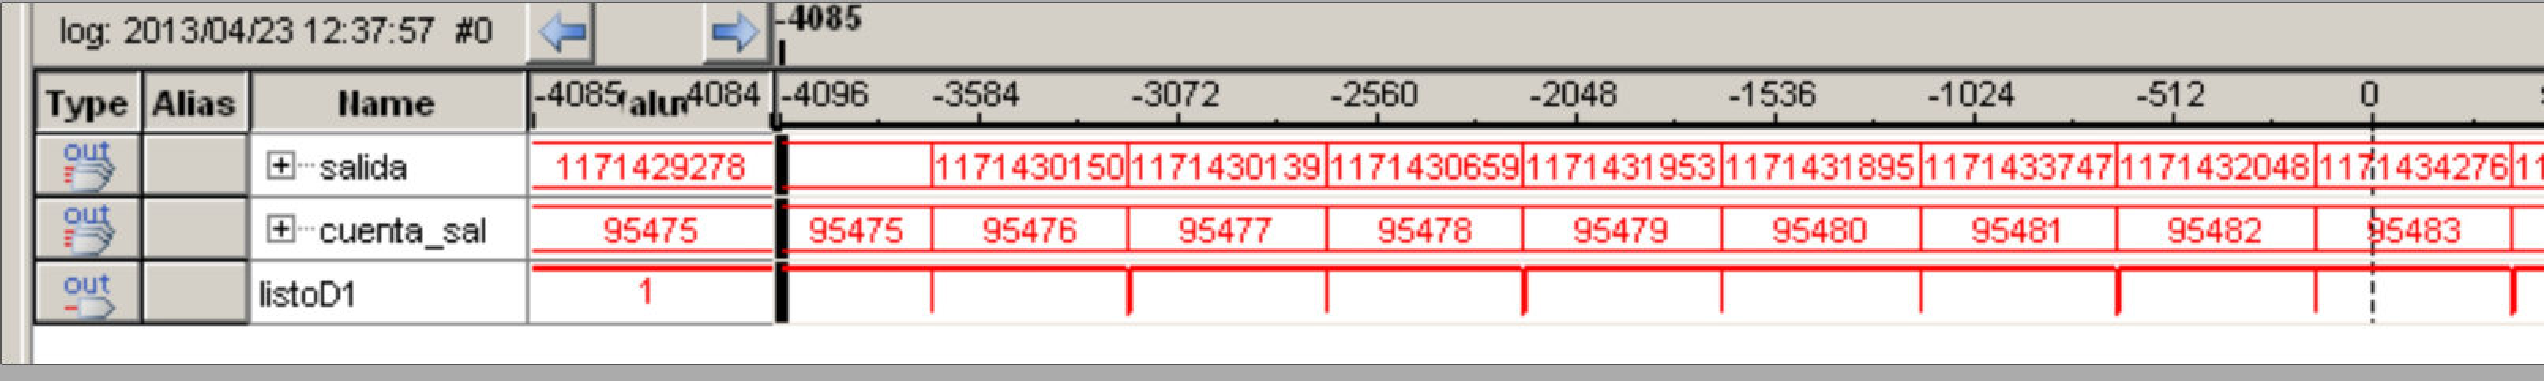
\includegraphics[width=1\columnwidth]{st.pdf}\\
	\caption{Salida del Signal Tap.}\label{fig:st}
\end{figure*}
%
\begin{figure}
	\centering
	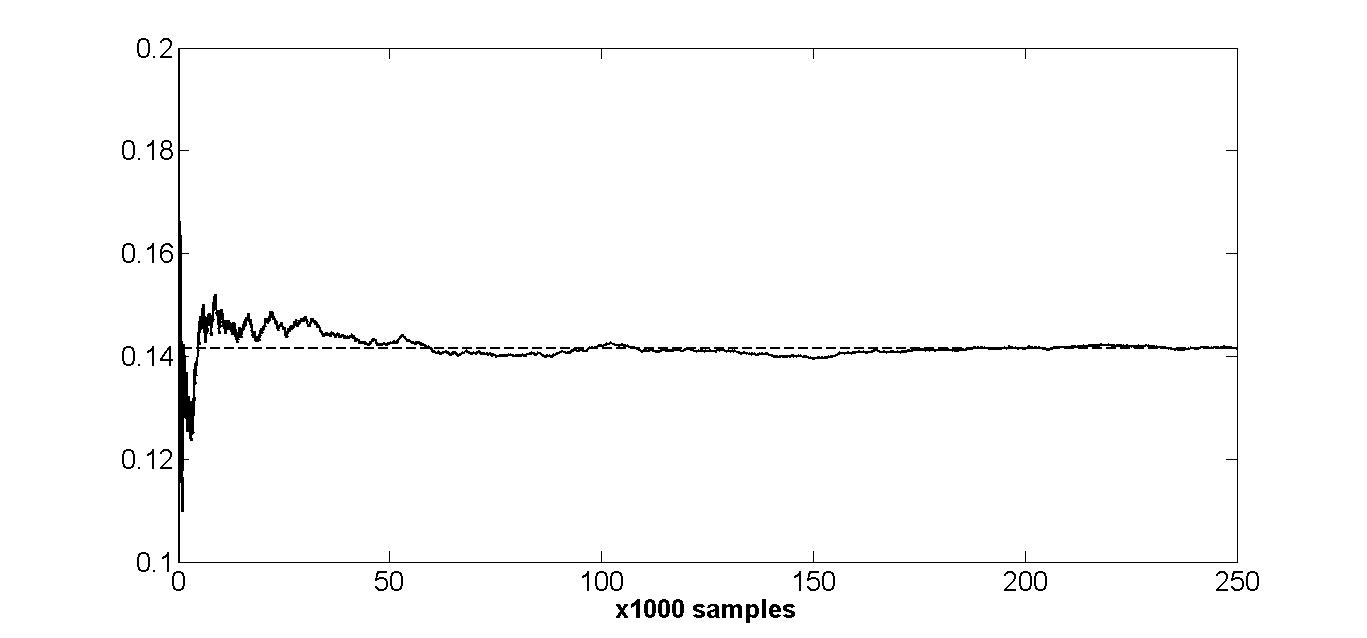
\includegraphics[width=1\columnwidth]{Lyap_MATLAB.jpg}\\
	\caption{Convergencia del algoritmo que calcula el MLE.}\label{fig:lyapu}
\end{figure}